\documentclass[a4paper]{scrreprt}

%% Language and font encodings
\usepackage[polish]{babel}
\usepackage[T1]{fontenc}

%% Sets page size and margins
\usepackage[a4paper,top=3cm,bottom=2cm,left=3cm,right=3cm,marginparwidth=1.75cm]{geometry}

%% Useful packages
\usepackage{amsmath}
\usepackage{graphicx}
\usepackage[colorinlistoftodos]{todonotes}
\usepackage[colorlinks=true, allcolors=blue]{hyperref}

\def \GameTiTle{Technocracy}
%Technokracja

\title{\GameTiTle{}}
\subtitle{Dokument projektowy wersja 1}
\author{Laura Stasiulewicz}

\titlehead{\centering}

\begin{document}
\maketitle

\begin{abstract}
\GameTiTle{} to gra strategiczna czasu rzeczywistego. Celem gracza jest pokonanie komputerowego przeciwnika w walce o kontrolę nad punktem dominacji na mapie. Aby to uczynić, musi wykorzystać zdolność planowania, zarządzania zarówno jednostkami, jak i zasobami oraz wiedzy na temat dostępnych rodzajów oddziałów jakie może przywołać i interakcji między nimi.  %Gracz wciela się w jedną z kilku frakcji kosmicznych osadników z Ziemi walczących między sobą o kontrolę nad odległą egzoplanetą. Ze względu na słabe pole magnetyczne, nieustającą wojnę oraz odległość od innych zamieszkałych ciał niebieski ich nowy świat stał się cmentarzyskiem, a główną ucieczka z niego ambicją jego mieszkańców. 
%Short abstract of the game (max 150 words) 

\end{abstract}

{
  \hypersetup{linkcolor=black}
  \tableofcontents
}

% ______________________
% chapter Overview
% ______________________
\chapter{Przegląd}
\GameTiTle{} to gra strategiczna czasu rzeczywistego. Akcja gry umiejscowiona jest w dalekiej przyszłości, w której kolonizacja kosmosu przez ludzi jest w zaawansowanym stopniu. Koloniści docierają i zdobywają  egzoplanety oddalone od ziemi o dekady świetlne. "Nowe światy" nie są jednak dla ludzkości błogim rajem, osadnicy szybko dzielą się na frakcje, między którymi dochodzi do nigdy niekończących się konfliktów. Gracz wciela się w przywódcę jednego z podobnych ugrupowań walczących o nad jedną z takich planet. Ze względu na słabe pole magnetyczne, ciągnących się przez tysiące lat wojen oraz odległość od innych zamieszkałych ciał niebieski ich nowy świat stał się cmentarzyskiem, a przetrwanie główną ambicją jego mieszkańców.
\section{Główny Zamysł}
Zamysł gry opiera się na klasycznej formule gier RTS \emph{(Real Time Strategy - ang. strategii czasu rzeczywistego)}. Ekran gry podzielony jest na mapę oraz nakładkę stanowiącą interfejs gracza. Gracz wydaje polecenia przy użyciu myszy oraz skrótów klawiaturowych. Rozgrywka polega na zdobywaniu punktów poprzez kontrolowanie odpowiednich sektorów na mapie. Aby to osiągnąć gracz musi budować odpowiednie struktury oraz oddziały, utrzymywać kontrolę nad ważnymi dla niego zasobami oraz tworzyć odpowiednią infrastrukturę do ich przetwarzania, co wymaga od niego umiejętności planowania i zmysłu strategicznego. Przeciwnikiem gracza jest sztuczna inteligencja, próbujące zrealizować identyczne cele.

\section{Co odróżnia mój tytuł?}
W ciągu ostatnich lat gry strategiczne podzieliły się na dwa rodzaje: skupiające się na rywalizacji rankingowej między ludzkimi przeciwnikami w rozgrywkach sieciowych, wymagające dużo czasu, zaangażowania i energii od graczy. Oraz ich kompletne przeciwieństwa, gry ekonomiczne z powolnym postępem oraz kompletnym brakiem lub mocno okrojoną warstwą militarną.
\GameTiTle{} ma być powrotem do korzeni, ma nawiązywać do pierwszych serii gier RTS, gdzie głównym elementem były potyczki z komputerowymi graczami oraz scenariusze do rozgrywania przez pojedynczego gracza. Dzięki temu osoby, które lubią formułę gier tego rodzaju, ale brak im czasu, aby osiągnąć, często wysoki, próg umiejętności do gry sieciowej mogły także się nią cieszyć. 
W \GameTiTle{} warstwa ekonomiczna ma być nie tylko równie ważna i angażujące, ale też równie rozbudowana co warstwa militarna.

% ______________________
% chapter References
% ______________________

\chapter{Odniesienia i inspiracje} 

\section{Seria \emph{Twierdza}, Firefly Studios}
Seria \emph{Twierdza} jest bezpośrednią 
inspiracją \GameTiTle{}. Podczas gdy ekonomia wielu gier w jej gatunku sprowadza się do postawienia budynku na źródle zasobu lub wysłaniu pracownika, który ma dany zasób zbierać, w serii Twierdza twórcy zaimplementowali proste łańcuchy dostaw i przetwarzania surowców, co nadaje rozgrywce dodatkowej głębi. Ponadto widok krzątających się postaci nadaje grze niepowtarzalnego klimatu oraz imersji. \GameTiTle{} pragnie wzbogacić te elementy dodając kompetentnego przeciwnika SI oraz wzbogacić grę o nowoczesne elementy interfejsu, sterowania oraz silnik pozwalający na lepszą fizykę obiektów w świecie gry.

\begin{figure}[hb]
\centering
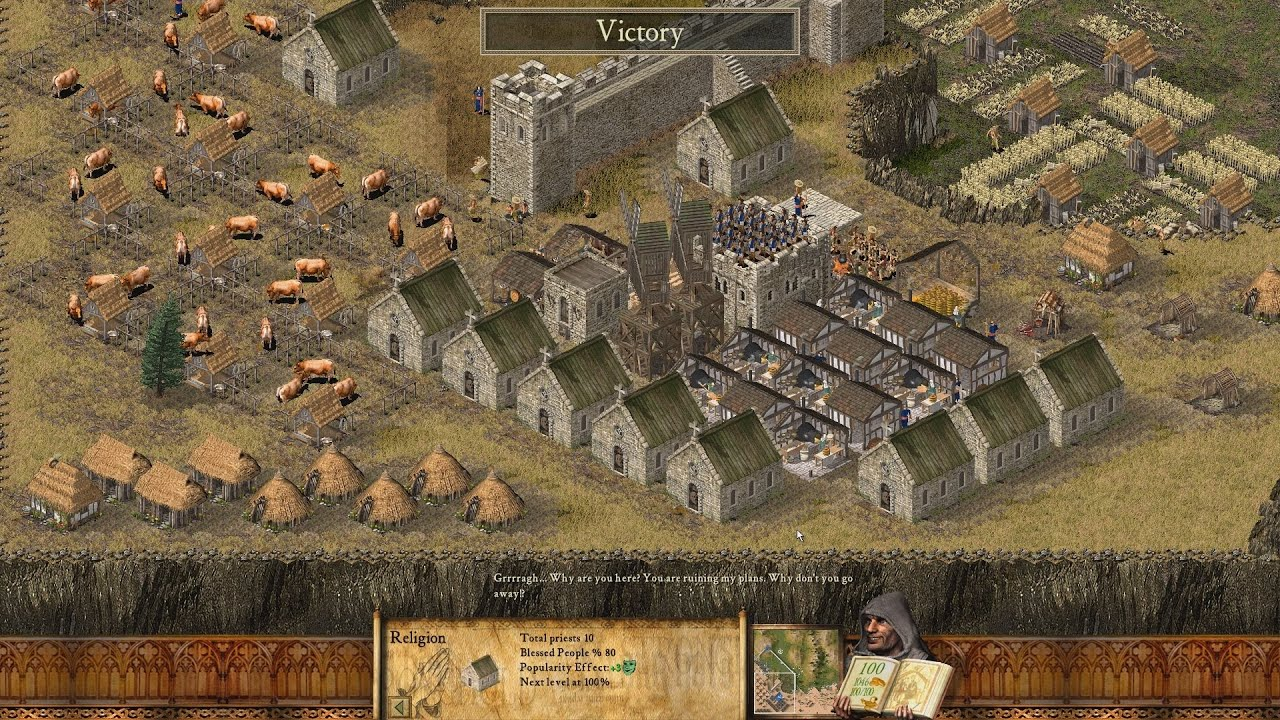
\includegraphics[width=1\textwidth]{stronghold2.jpg}
\caption{\label{} Zrzut ekranu z gry Twierdza}
\end{figure}
\newpage

\section{Seria \emph{Company of Heroes}, Relic Entertainment}
Seria \emph{Company of Heroes} odznaczyła się nie tylko poprzez doskonale rozwinięty tryb sieciowy, ale także poprzez dużo ilość zawartości dla pojedynczego gracza oraz za ikoniczny tryb walki nad sektorami zwycięstwa. Ważnym elementem rozgrywki była doktryna sił połączonych: gracz musiał umiejętnie dopierać kompozycję swojej armii, aby móc odpowiadać na ataki przeciwnika. 
W \GameTiTle{} te elementy wprowadzimy na własny sposób, łącząc taktyczne aspekty serii z bardziej rozbudowaną warstwą ekonomiczną.

\begin{figure}[hb]
    \centering
    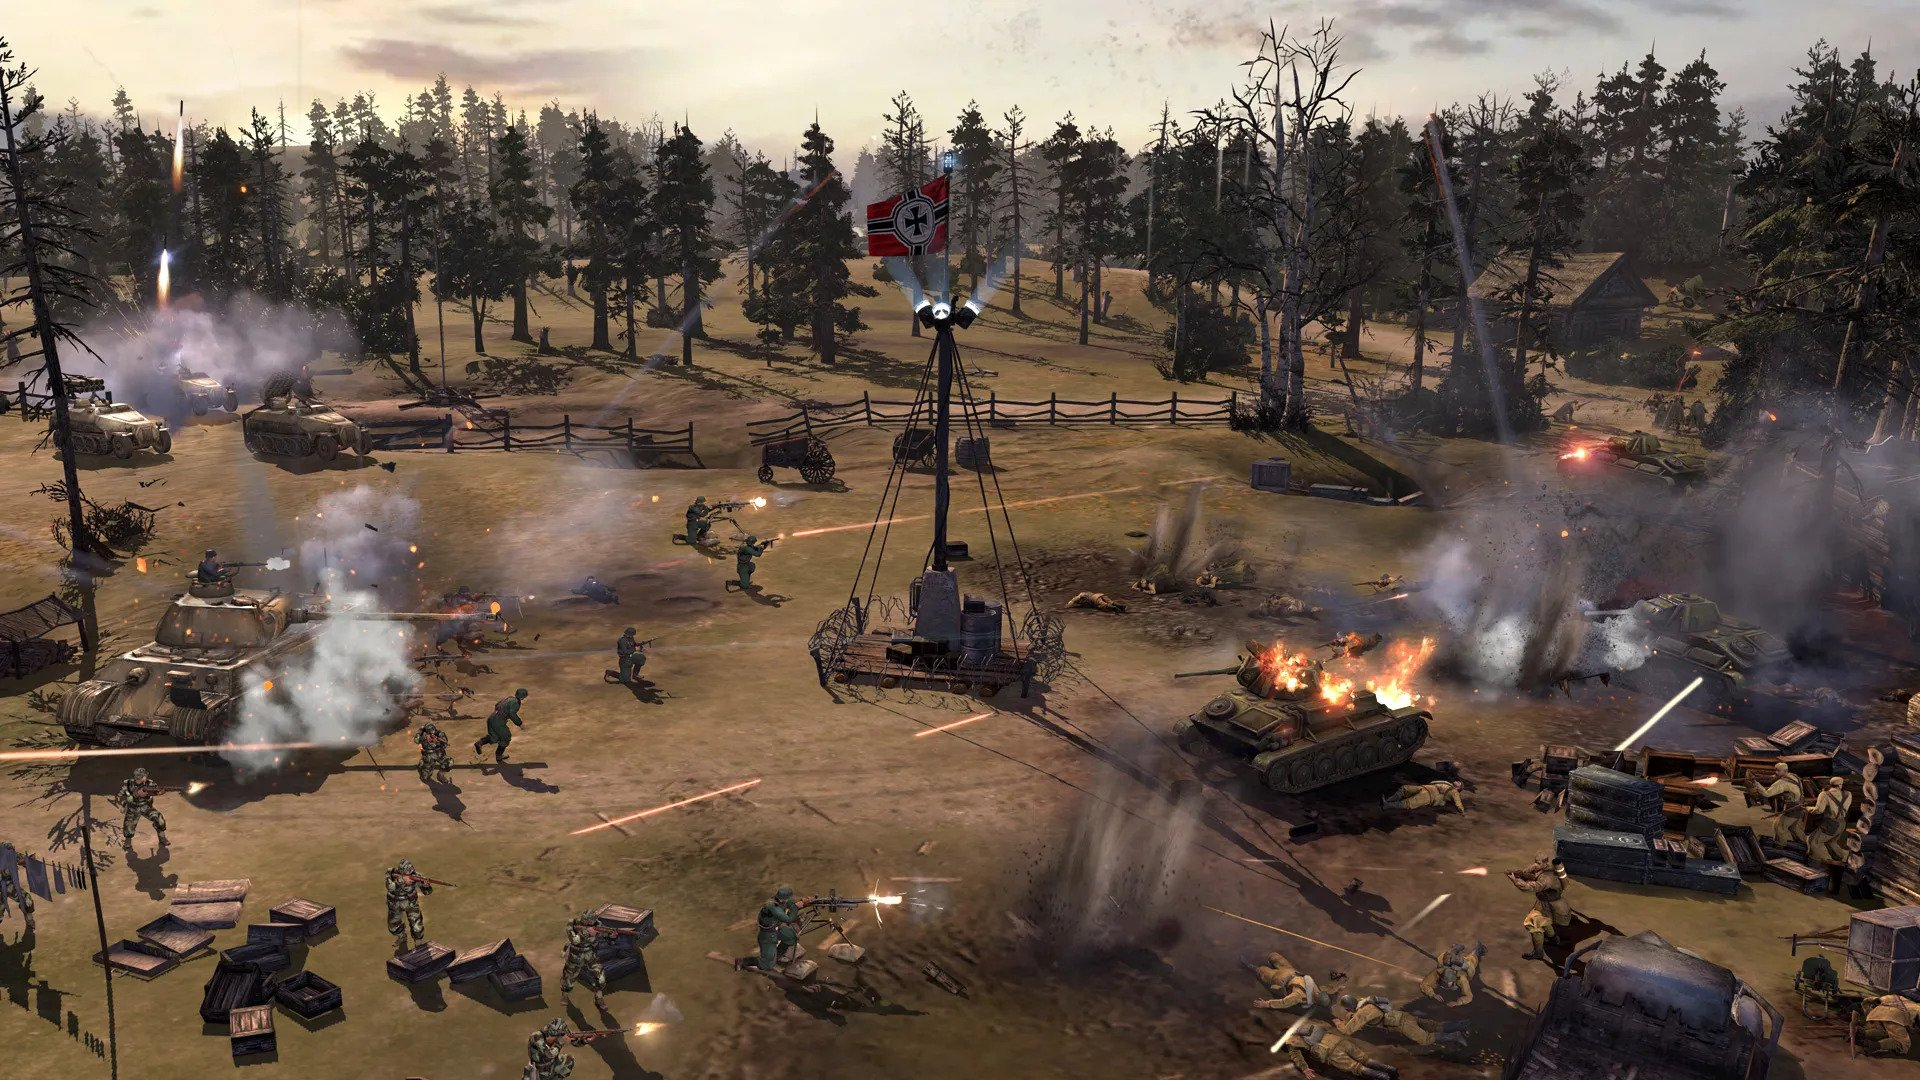
\includegraphics[width=1\textwidth]{coh2.jpg}
    \caption{\label{} Walka o sektor kontrolny w grze Company of Heroes 2}
    \end{figure}

% ______________________
% chapter Specification and Market Analysis 
% ______________________

\chapter{Szczegóły techniczne}
%description of target group, platform, art style, who to attract of how to attract 

\section{Grupa docelowa}
Osoby po 18 roku życia, fani klasycznych strategii, osoby, które spędzają średnio od 3 do 12 godzin tygodniowo na graniu w gry komputerowe. Gra ma ich przyciągnąć niskim progiem umiejętności potrzebnym do wejścia do gry, stosunkowo krótkim czasem pojedynczej rozgrywki, tak aby osoby z grupy docelowej miały czas w nią grać, a w wypadku przegranej, miały mniejsze poczucie frustracji.

\section{Gatunek}
Gra należy do gatunku strategii czasu rzeczywistego.
\section{Styl graficzny}
Gra będzie wykorzystywać grafikę 2D, z wykorzystaniem techniki \emph{Pixel Art.}

\begin{figure}[hb]
\centering
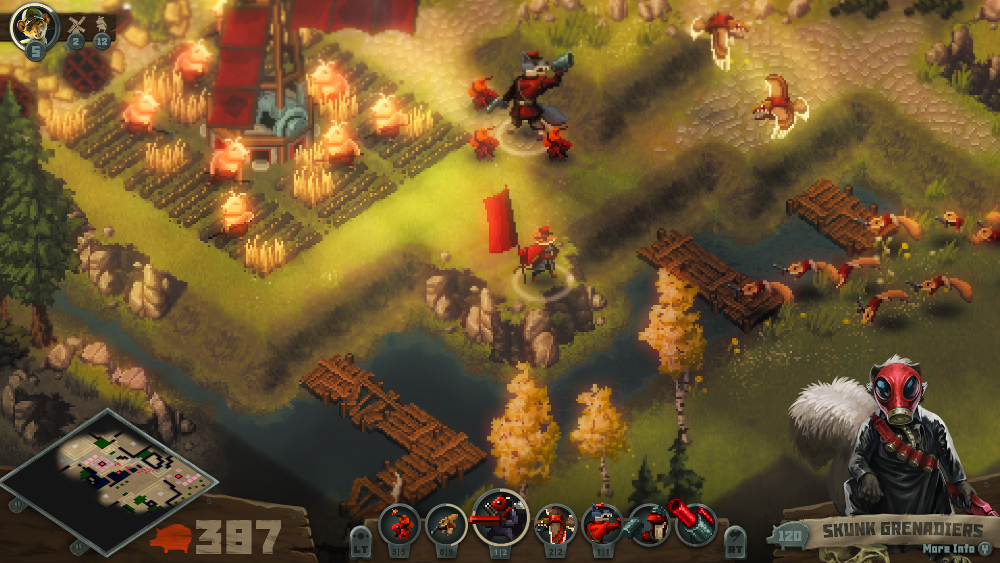
\includegraphics[width=1\textwidth]{ToothAndTail.png}
\caption{\label{fig:arteg1} Przykład grafiki w stylu Pixel Art (Tooth and Tail, Pocketwatch Games)}
\end{figure}

% \begin{figure}[hb]
%   \centering
%   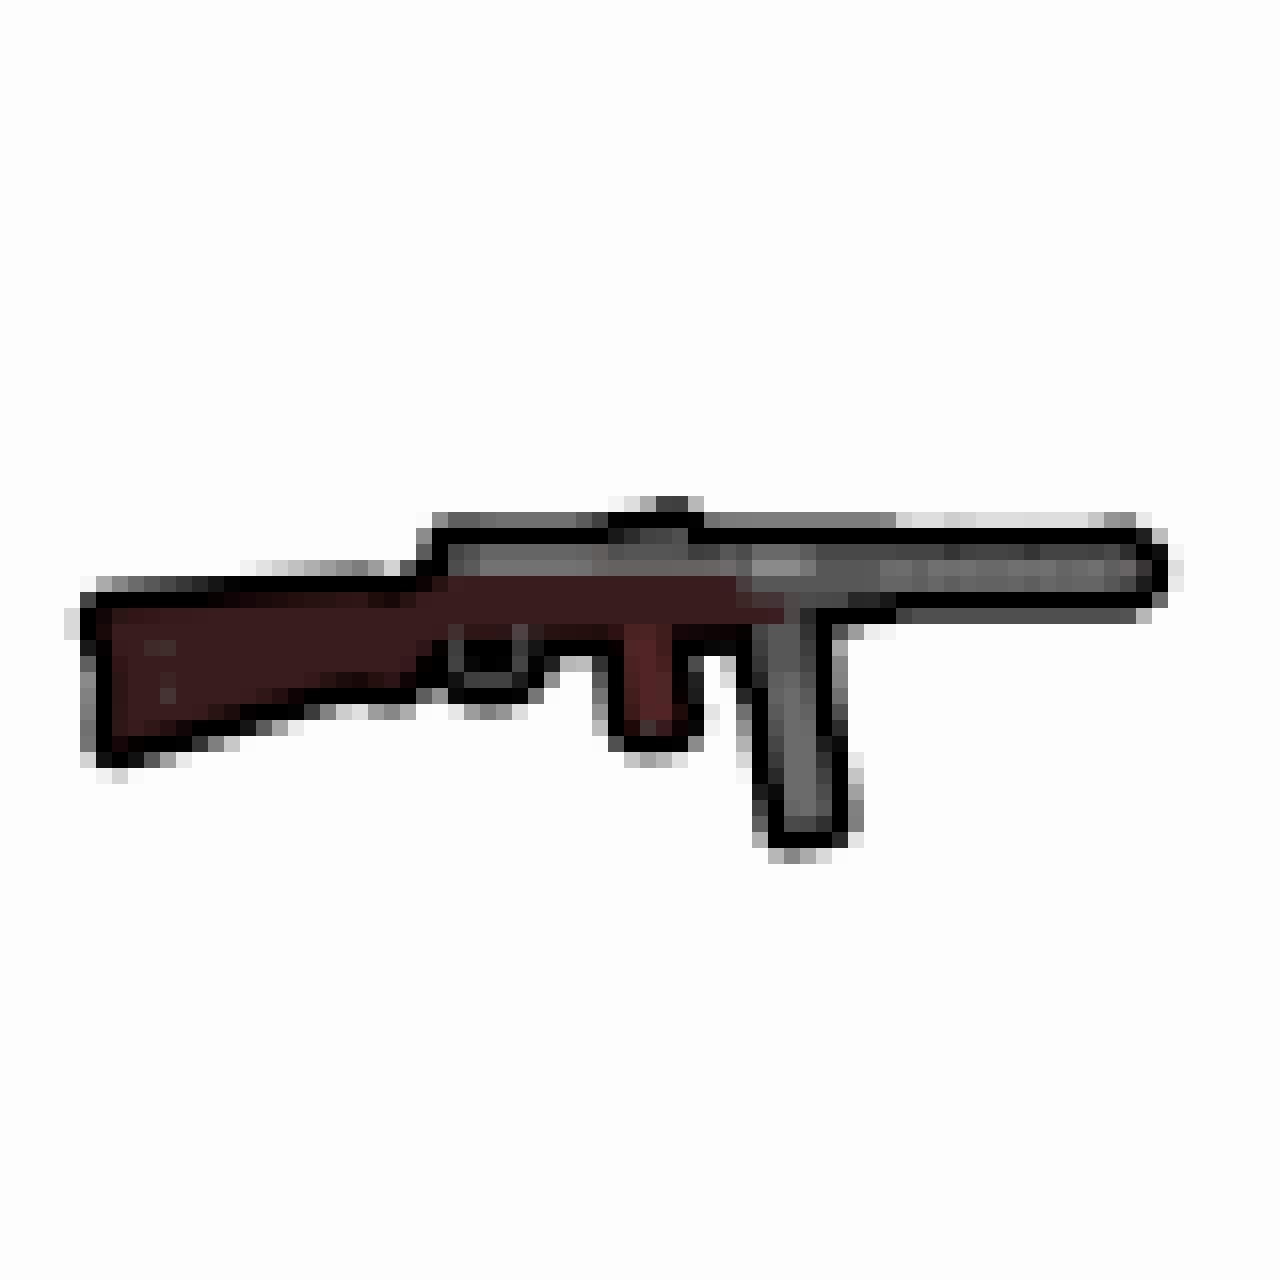
\includegraphics[width=0.6\textwidth]{morswpng.png}
%   \caption{\label{fig:arteg2} Przykład grafiki wykonanej w stylu Pixel Art}
%   \end{figure}


\section{Formy Zaangażowania Gracza}
%thinking of Hunicke's 8 kinds of "fun" - what would you like to focus on?\\
% (1. Sensation - Game as sense-pleasure 
% 2. Fantasy - Game as make-believe
% 3. Narrative - Game as drama
% 4. Challenge - Game as obstacle course
% 5. Fellowship -  Game as social framework
% 6. Discovery - Game as uncharted territory 
% 7. Expression - Game as self-discovery 
% 8. Submission - Game as pastime)
\GameTiTle{} pozwala graczowi sprawdzić się w wyzwaniu, jakim będzie pokonanie przeciwnika SI. Będzie musiał to tego wykorzystać zarówno zręczność, jak i umiejętność strategicznego myślenia. Gracz może się wczuć w postapokaliptyczny konflikt, poprzez warstwę wizualną i fabułę.
% ______________________
% chapter Game Details
% ______________________


\chapter{Gameplay i Umiejscowienie Rozgrywki}
%be specific about the core game features 

% \section{Nastrój oraz Emocje}
% what mood and emotions does the game create (can change e.g. for every level / section) 

% \section{Story}
% the story of the game

\section{Świat Przedstawiony}
Gra umiejscowiona jest w dalekiej przyszłości, na fikcyjnej planecie. Została ona skolonizowana przez ludzi tysiące lat temu, jednak millenia konfliktów zbrojnych oraz szczególnie nieprzyjazne warunki spowodowały, że ziemscy osadnicy utracili technologię, z którą przybyli do tego nowego świata. Walki toczą się o bogate w zasoby i technologię schrony i ruiny zbudowane przez pierwszych osadników w czasach ich świetności.

\section{Przykładowa Mapa Rozgrywki}
Potyczki między graczem a SI będą się rozgrywać na różnorodnych mapach. Każda mapa rozgrywki powinna posiadać 3 sektory kontrolne. Dostęp do nich jest ograniczony poprzez rozmieszone niedostępne obszary, przez co w trakcie rozgrywki wydzielają się "korytarze" o różnej szerokości, faworyzując bardziej defensywny styl gry w węższych "korytarzach".
Kluczowe strategiczne zasoby są umiejscowione blisko centrum akcji, co ma skłaniać graczy do prób zablokowania tych zasobów dla przeciwnika.
\begin{figure}[hb]
  \centering
  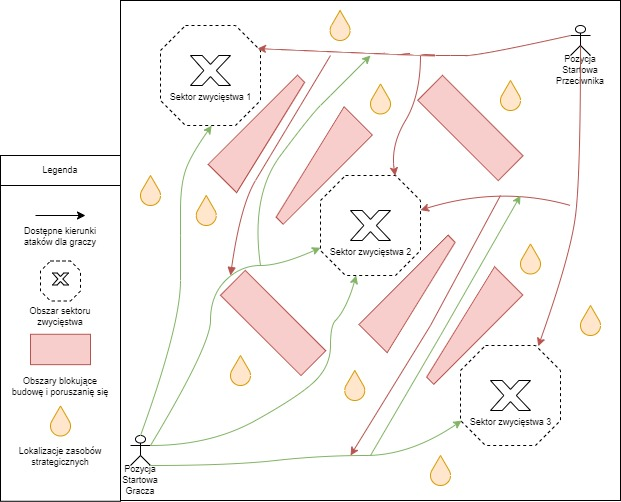
\includegraphics[width=1\textwidth]{exampleMap.jpg}
  \caption{\label{fig:map1} Schemat przykładowej mapy rozgrywki}
  \end{figure}

\section{Obiekty}
W świecie gry można wyróżnić trzy główne rodzaje obiektów:
\subsection{Budynki}
Statyczne obiekty umieszczane przez gracza lub przeciwnika komputerowego. Gracz może wybierać budynki oraz wydawać im polecenia. Obiekty tego rodzaju mogą ulec zniszczeniu w trakcie rozgrywki. Budynki posiadają szereg interakcji z innymi obiektami, np. atak, zmagazynowanie surowca w budynku, etc. Gracze mogą rozpocząć grę z kilkoma tego typu obiektami już pod ich kontrolą.
\subsection{Oddziały i Pracownicy}
Obiekty te mogą poruszać się po mapie, podlegają bezpośredniej kontroli gracza, Obiekty tego rodzaju można niszczyć. Oddziały mają charakter militarny, ich głównym zdaniem jest atakowanie obiektów przeciwnika. Pracownicy mają charakter cywilny, polecenia, jakie gracz może im wydawać związane są z wydobywaniem zasobów oraz budowaniem budynków.
\subsection{Obiekty otoczenia}
Statyczne obiekty nienależące do żadnej frakcji, takie jak drzewa, złoża zasobów, ruiny, wraki etc. 

\section{Cel Gry}
Gra opiera się o potyczki z przeciwnikiem SI. Na mapie rozmieszczone są sektory kontroli. Zdobywa się je poprzez budowę specjalnego obiektu w obrębie strefy. Strona posiadająca więcej stref kontroli zdobywa punkty. Tempo ich zdobywania rośnie wraz z przewagą w przejętych strefach kontroli. Strona, która jako pierwsza osiągnie limit punktów, wygrywa. Analogicznie, jeżeli gracz zbierze mniejszą ilość punktów, następuje jego przegrana. Przegrana następuje również wtedy, gdy wszystkie budynki produkcyjne jednego z graczy zostaną zniszczone.
\section{Główne mechaniki}
\subsection{Zbieranie surowców}
Surowce w grze zbierane są poprzez budynki budowane w pobliżu ich złóż. Z budynków wychodzą pracownicy, którzy wydobywają surowiec i zanoszą go z powrotem do budynku. Gdy magazyn budynku się zapełni, pracownik  tragarz rusza z ładunkiem do innego budynku pełniącego funkcję magazynu. Następnie surowiec jest dalej przetwarzany, zanoszony z powrotem do magazynu i w takiej postaci może być wykorzystany do budowy jednostek budynków, etc.
\subsection{Budowa budynków} 
Gracz zleca budowę budynku poprzez wybranie jednostki, następnie z menu akcji jednostki wybiera opcję budowy budynku, a następnie rodzaj budynku, jaki chce umieścić. 
\subsection{Budowa jednostek}
Gracz zleca budowę jednostki poprzez wybranie budynku, następnie z menu akcji obiektu wybiera opcję budowy budynku, a następnie rodzaj jednostki, jaką chce zbudować. 
\subsection{Walka}
Większość oddziałów atakuje wroga przy pomocy ataków dystansowych. Ataki mogę być bezpośrednie (jeden atak zadaję obrażenia jednemu przeciwnikowi) lub obszarowe (jeden atak zadaje obrażenia wszystkim przeciwnikom w danym obszarze). Jednostki dzielą się na kilka klas, pomiędzy którymi panują zależności na analogicznej zasadzie co w grze \emph{papier, kamień, nożyce}. Niektóre klasy jednostek są bardziej lub mniej skuteczne w walce z innymi jednostkami. Zachęca do gracza do budowania armii o zróżnicowanej kompozycji i sprawia, że każda jednostka na zastosowanie w grze.
\subsection{Kontrola nad sektorami}
W centrum każdego sektora znajduję się specjalny obiekt-gniazdo, na którym można umieść budynek dający kontrolę nad sektorem. Gracz (człowiek lub jego przeciwnik SI), który postawi budynek, przejmuje kontrole nad sektorem. 
\section{Sterowanie}
Gra do sterowania wykorzystuje mysz oraz skróty klawiaturowe. Przy pomocy mysz gracz steruje kamerą, wydaje polecenia jednostkom na mapie oraz wybiera lokalizację budynków.
Skróty klawiaturowe można dostosować w opcjach gry.
% ______________________
% chapter Front End
% ______________________


\chapter{Interfejs}
W poniższym rozdziale omówione są elementy interfejsu. 
\section{Schemat przejść między ekranami}

\begin{figure}[hb]
  \centering
  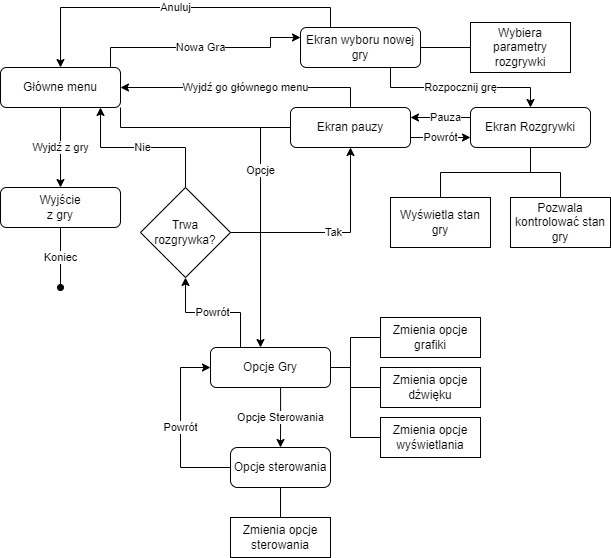
\includegraphics[width=1\textwidth]{screenDiagram.jpg}
  \caption{\label{fig:schema1} Schemat przejść pomiędzy poszczególnymi ekranami gry}
\end{figure}
\newpage

\section{Ekran rozgrywki}
\begin{figure}[hb]
  \centering
  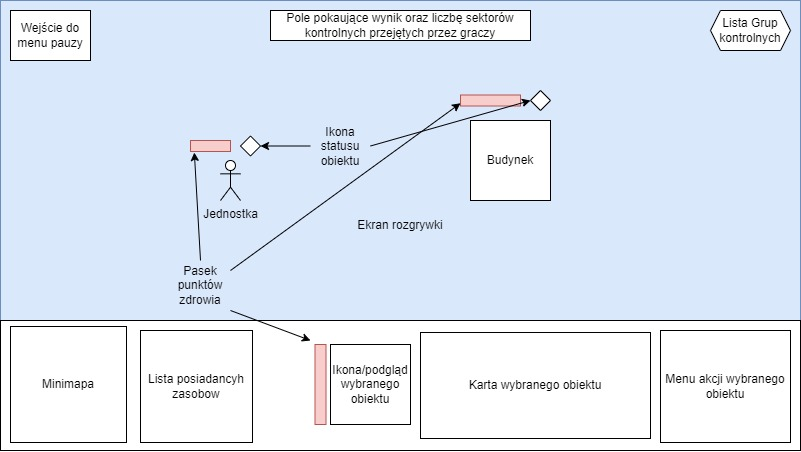
\includegraphics[width=1\textwidth]{mainScreenExample.jpg}
  \caption{\label{fig:schema2} Schemat przejść pomiędzy poszczególnymi ekranami gry}
\end{figure}

% ______________________
% chapter Game Details
% ______________________


\chapter{Wykorzystane Technologie}
% what technologies is the game designed for, what is the target platform, what technologies are used for the development? 

\section{Docelowe systemy}
Komputery z systemem operacyjnym Windows.

\section{Wymagania sprzętowe}
Do późniejszego ustalenia.

\section{Używane narzędzia}
\begin{itemize}
  \item Silnik gry: Unity 2022.1.1.6f1
  \item Edytory graficzne: Krita, Pixelorama
  \item IDE: Microsoft Visual Studio 2022, Unity Editor
\end{itemize}

% ______________________
% chapter Game Details
% ______________________


% \chapter{Topic and Inclusion }

% describe here how you plan to address the main topic (main theme) and topics around inclusion

% \section{Main Theme}
% \section{Inkluzywność}

% \subsection{Rożnorodność}
% diversity in games is an important topic. please describe here how you addresses diversity in your game and game design elements 
% \subsection{Dostępność}
% make your games more accessible. use this section to describe what guidelines you addresses and how you cater for  gamers with disabilities and other impairments. great reference: \url{http://gameaccessibilityguidelines.com/}
% %\subsection{Humanity}

% ______________________
% chapter Game Details
% ______________________


% \chapter{Timeline and Cost Estimation}

% In this chapter, you should describe your planned time management, the estimation of how long you think your team will need and how much you think this project would cost. 

% Tools we recommend for project management are for instance \url{https://app.hacknplan.com/login}. To track your time, we recommend \url{https://toggl.com/}.  

% \begin{table}[h]
% \centering
% \begin{tabular}{|l|l|l|}
% \hline
% Milestone & Description & Date \\\hline
% & Official Start Date & 01.12.... \\
% 1 & Milestone Description ..  & 01.12.... \\
% 2 & Milestone Description ..  & 01.01.... \\
% 3 & Milestone Description ..  & 01.03.... \\
% & End of Project & 01.04.... \\
% \hline
% \end{tabular}
% \caption{\label{tab:schedule}Example Schedule.}
% \end{table}

% \section{Time Estimation}

% While working on your project you should track your time. 
% We recommend using \url{https://toggl.com/} for time management. In the final report you will have to compare the estimated time with the actual time. (Miscalculation do not have any effect on your grade!!!)

% \section{Cost Estimation}

% Estimated cost of the project based the described tasks and milestones and the  time estimation.  

% ______________________
% chapter Game Details
% ______________________


\chapter{Zespół}
Laura Stasiulewicz - design, grafika, programowanie

% Additional Credits (e.g. sources of art, audio,.. ) 

% \todo[inline, color=green!40]{This is an inline comment.}

%\bibliographystyle{alpha}
%\bibliography{sample}

\end{document}